% LaTeX Article Template - customizing header and footer
\documentclass{article}

\newtheorem{thm}{Theorem}

% Set left margin - The default is 1 inch, so the following
% command sets a 1.25-inch left margin.
\setlength{\oddsidemargin}{0.25in}

% Set width of the text - What is left will be the right margin.
% In this case, right margin is 8.5in - 1.25in - 6in = 1.25in.
\setlength{\textwidth}{6in}

% Set top margin - The default is 1 inch, so the following
% command sets a 0.75-inch top margin.
\setlength{\topmargin}{-0.25in}

% Set height of the header
\setlength{\headheight}{0.3in}

% Set vertical distance between the header and the text
\setlength{\headsep}{0.2in}

% Set height of the text
\setlength{\textheight}{9in}

% Set vertical distance between the text and the
% bottom of footer
\setlength{\footskip}{0.1in}

% Set the beginning of a LaTeX document
\usepackage{multirow}
\usepackage{fullpage}
\usepackage{graphicx}
\usepackage{amsthm}
\usepackage{amssymb}
\usepackage{amssymb}
\usepackage{algpseudocode}
\usepackage{listings}
\usepackage{color}
\usepackage{float}


\definecolor{dkgreen}{rgb}{0,0.6,0}
\definecolor{gray}{rgb}{0.5,0.5,0.5}
\definecolor{mauve}{rgb}{0.58,0,0.82}

\lstset{frame=tb,
  language=python,
  aboveskip=3mm,
  belowskip=3mm,
  showstringspaces=false,
  columns=flexible,
  basicstyle={\small\ttfamily},
  numbers=none,
  numberstyle=\tiny\color{gray},
  keywordstyle=\color{blue},
  commentstyle=\color{dkgreen},
  stringstyle=\color{mauve},
  breaklines=true,
  breakatwhitespace=true,
  tabsize=3
}

\graphicspath{%
    {converted_graphics/}% inserted by PCTeX
    {/}% inserted by PCTeX
}
%%%%%%%%%%%%%%%%%%%%%%%%%%%%%

\begin{document}\title{Homework $1$\\ Computer Science \\ Spring 2017\\ B351}         % Enter your title between curly braces
\author{Steven Myers}        % Enter your name between curly braces
\date{\today}          % Enter your date or \today between curly braces
\maketitle


% Redefine "plain" pagestyle
\makeatother     % `@' is restored as a "non-letter" character


% Set to use the "plain" pagestyle
\pagestyle{plain}
All the work herein is mine.

\section*{Answers}

\begin{enumerate}
    \item % problem one
    Here are the definitions for the terms listed in Problem 3.10:
    \begin{enumerate}
        \item \textbf{State} - A particular assignment of value to all variables for a given situation.
        \item \textbf{State space} - All of the possible assignments of values to variable in a scenario.
        \item \textbf{Search tree} - An arrangement of states such that no state is repeated twice when traversing all states.
        \item \textbf{Search node} - A particular node in a search tree that has a cost and ingoing or outgoing paths. Each node contains the cost of the current node, its data (state values), and the cost of visiting other accessible states.
        \item \textbf{Goal} - A final search node with an ideal or target state that we want to obtain to resolve a problem.
        \item \textbf{Action} - An operation that results in a change of state.
        \item \textbf{Transition model} - The process of moving from one state to another when an action is applied.
        \item \textbf{Branching factor} - The maximum number of "branches" or pathways that some search node can have. This is used to limit the search space and prevent a machine from running out of memory before resolving a problem when the search space is too large.
    \end{enumerate}
    \item % Describe a state space in which iterative deepening search performs much worse than depth-first search (for example, O(n2) vs. O(n)).
    A state space where iterative deepning search would perform worse than DFS is one in which the following are true:
    \begin{enumerate}
        \item The branching factor is large.
        \item The depth of each branch is shallow, and the goal node exists in a branch which is deeper than the others.
    \end{enumerate}
    A state space such as Figure 1 could produce a circumstance where DFS would perform significantly better than iterative deepening search.
    \begin{figure}[H]
        \centering
        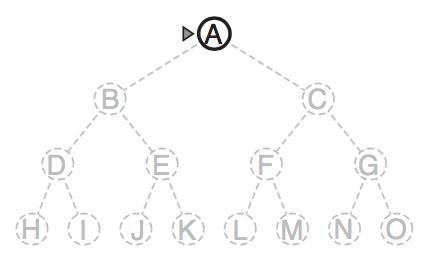
\includegraphics[width=.5\linewidth, height=.15\textheight]{dfs_example}
        \caption{Attach a goal node \textbf{S} as a node \textbf{O}'s right child. (Image taken from textbook figure 3.16 on page 86, Russel \& Norvig)}
    \end{figure}
    \item Yes, the graph is consistent. Here are the statements for each node and its sucessors:
    \begin{enumerate}
        \item AB: $1 \leq 6$
        \item AC: $1 \leq 8$
        \item BC: $4 \leq 4$
    \end{enumerate}
    \item
    \begin{enumerate}
        \item Solution in \texttt{rv1.py}. Reads in the file \texttt{f.txt} and outputs the directions in \texttt{directions.txt} if a path exists from the robot's starting point to the goal position.

        \item Better solution in \texttt{rv2.py}. Reads in the file \texttt{f.txt} and outputs the directions in \texttt{directions2.txt} if a path exists from the robot's starting point to the goal position. I used BFS to determine the shortest path from the current tile to the goal node. BFS is guaranteed to find the shortest path since it traverses the graph in a similar way that the robot would do so (one tile in a cardinal direction at a time). This is because my adjacent function only returns tiles NWES of the current tile and not in the diagonal directions. Once I got the shortest path from BFS, I made my robot traverse the path and rotate as necessary and recorded the steps.

        \item In \texttt{rv1.py}, I created a very simple search that essentially models the robot randomly exploring the entire maze, always turning left when given the opportunity. So, it's as if the robot walks along the wall with its left hand on the wall and turns around at every dead-end. It explores the entire maze (perhaps the most inefficient path, depending on the maze layout). This search \textbf{fails} when the maze contains cycles, and will incur an infinite loop since the robot will wander forever. If there is no path from the robot's starting point to its goal node, then the robot's path finding function will return false. This is done by doing a DFS search from the robot's starting position and looking to see whether or not the goal position is reachable.
        \\\\
        In \texttt{rv2.py}, I used BFS to find the shortest path then made the robot follow that path, rotating as needed. This search also \textbf{fails} when the maze contains cycles. If the BFS search did not yield a path to the goal node, the program halts and errors out as no path exists.
        \\\\
        In both of my files, the $g(n)$ or weight of the edges is equivalent since all edges that are connected are exactly one tile away. The $h(n)$ or cost to reach the goal node from any given node is calculated based on its order in the shortest path. So, every node on the path to the goal node is exactly one node cheaper than the previous node. No shortest path requires more than one rotation by the robot at any given point, so we can say that the cost of intersections is also uniform throughout the entire graph.


    \end{enumerate}
    \item I extended the rock, paper, scissors game from the last homework assignment. The file is included as \texttt{rpgs.py} as requested. This version of the game differs from the previous version since the computer and the human take bets. There is more human-interaction with the game, as you must decide when you should take bets, etc. The computer takes bets based on whether or not it's on a losing or winning streak. You lose the game if you run out of money (less than 10 dollars), and win the game if the computer runs out of money.
\end{enumerate}
\end{document}
